\graphicspath{{figures/chap05/}}

\chapter{结论、课题工作存在的不足与后续工作展望}
\label{chap:summary}

%本文工作围绕在 SUNIST 球形托卡马克上建立氦原子发射光谱强度比诊断电子温度和电子密度手段开展。做为托卡马克高温等离子体的一种非侵入式诊断手段,可见光波段的原子光谱发射诊断具有不干扰等离子体、测量设备简单、不易受托卡马克复杂电磁环境影响以及易实现时间和空间分辨测量的优点,并且在设备总装后,可以实现少维护甚至是免维护。而氦原子本身的特性使得氦原子谱线辐射在托卡马克聚变等离子体研究中受到了充分重视:1)氦原子具有两套自旋能级系统,自旋三重态只能通过电子碰撞自旋变化激发过程产生,其反应速率系数与自旋守恒激发过程具有不同的随电子温度变化趋势,这样通过测量来自不同自旋系统的三条谱线,即可以同时确定等离子体的电子温度与电子密度;2)氦原子具有最高的第一电离能,在大型托卡马克装置中,用氦原子束发射光谱法诊断时,测量粒子束可以深入到更深的等离子体位置甚至是中心区域;3)氦为聚变产物之一,在未来聚变装置中,利用氦原子的谱线辐射进行诊断不会为等离子体带来新的杂质。
%
%根据原子谱线辐射强度比分析出电子温度和密度信息的过程是以碰撞辐射模型对对应激发态粒子数密度的预测为基础的。一般情况下,碰撞辐射模型中只要包含了足够多的粒子数、反应过程和影响粒子数密度的其它相关效应,通过对各粒子数密度反应速率方程进行求解,即可以获得精确的能级数密度结果。
%
%由于现阶段原子反应过程速率系数的精度得不到保证,在碰撞辐射模型中包含跟多的粒子数时,却不能如预期的那样得到更高精度的结果。碰撞辐射模型中包含着数目巨大的激发态能级和复杂的相关反应过程,且各粒子之间通过原子反应相互关联,这样,目前并没有有效的手段对速率系数不确定性至激发态数密度计算误差之间的传递进行计算。通常的做法是通过对某反应过程的速率系数进行干扰,并重新求解碰撞辐射模型,以获得该速率系数的不确定性对粒子数密度计算的影响,这种方法并不直观,无法给出速率系数不确定性至激发态数密度计算误差传递之间的物理意义,且每次都要对碰撞辐射模型进行重新求解,也不能对速率系数精度提出具体的要求。
%
%实际研究中,碰撞辐射模型中包含更多能级粒子数时,并不能获得更高精度的结果。那么在特定的等离子体条件下,碰撞辐射模型中包含什么样的粒子和能级就可以获得可接受的计算结果成为了研究重点之一。在低温等离子体领域,人们发现在碰撞辐射模型中包含最主要的激发态能级粒子和反应过程,并结合实验对碰撞辐射模型的验证,可以对碰撞辐射模型进行简化,且可以得到满足实验精度要求的激发态能级粒子数密度计算结果。

本论文围绕 SUNIST 球形托卡马克装置上光谱诊断手段的建立,开展了氦放电等离子体原子发射光谱诊断电子温度和密度的研究。

做为托卡马克高温等离子体的一种非侵入式诊断手段,可见光波段的原子光谱发射诊断具有不干扰等离子体、测量设备简单、不易受托卡马克复杂电磁环境影响、易实现时间和空间分辨测量、系统总装后可实现少维护甚至是免维护等优点。而氦原子本身的特性,如两套自旋能级系统具有同时测量电子温度和密度的可能性、高电离能、本身是聚变产物之一等,使得氦原子谱线辐射在托卡马克聚变等离子体研究中受到了充分重视。

根据原子谱线辐射强度比分析出电子温度和密度信息的过程是以碰撞辐射模型对对应激发态粒子数密度的预测为基础的。一般情况下,碰撞辐射模型中只要包含了足够多的粒子数、反应过程和影响粒子数密度的其它相关效应,通过对各粒子数密度反应速率方程进行求解,即可以获得精确的能级数密度结果。

但是,由于现阶段原子反应过程速率系数的精度得不到保证,在碰撞辐射模型中包含更多的粒子数时,却不能如预期的那样得到更高精度的结果。碰撞辐射模型中包含着数目巨大的激发态能级和复杂的相关反应过程,且各粒子之间通过原子反应相互关联,这样,目前并没有有效的手段对速率系数不确定性至激发态数密度计算误差之间的传递进行计算。通常的做法是通过对某反应过程的速率系数进行干扰,并重新求解碰撞辐射模型,以获得该速率系数的不确定性对粒子数密度计算的影响,这种方法并不直观,无法给出速率系数不确定性至激发态数密度计算误差传递之间的物理意义,且每次都要对碰撞辐射模型进行重新求解,也不能对速率系数精度提出具体的要求。

因此,实际研究中,在特定的等离子体条件下,碰撞辐射模型中包含什么样的粒子和能级就可以获得可接受的计算结果成为了研究重点之一。在低温等离子体领域,人们发现在碰撞辐射模型中包含最主要的激发态能级粒子和反应过程,并结合实验对碰撞辐射模型的验证,可以对碰撞辐射模型进行简化,且可以得到满足实验精度要求的激发态能级粒子数密度计算结果。

%氦原子谱线比法的等离子体电子温度与密度参数范围与 SUNIST 等离子体相符(第 \ref{sec:ketiyiyi} 节)。做为一台小型球形托卡马克实验装置,SUNIST 需要发展不干扰等离子体、代价低、易用和尽量少维护的等离子体参数诊断手段,且 SUNIST 具有实验安排灵活的优势,适合进行诊断原理的验证性研究。基于以上考虑,为了解决碰撞辐射模型研究中存在的问题,本文在 SUNIST 上进行了氦原子发射光谱法诊断等离子体电子温度与密度手段的研究。

氦原子谱线比法的等离子体电子温度与密度参数范围与 SUNIST 等离子体相符(图 \ref{fig:chap01:te-ne-range})。做为一台小型球形托卡马克实验装置,SUNIST 需要发展不干扰等离子体、代价低、易用和尽量少维护的等离子体参数诊断手段,且 SUNIST 具有实验安排灵活的优势,适合进行诊断原理的验证性研究。基于以上考虑,为了解决碰撞辐射模型研究中存在的问题,本文在 SUNIST 上进行了氦原子发射光谱法诊断等离子体电子温度与密度手段的研究,这不仅对于完善 SUNIST 诊断有重要意义,也对氦原子光谱诊断方法的研究发展及其在未来聚变研究中的应用有积极意义。

\section{课题完成的工作和创新点}

碰撞辐射模型和谱线比诊断方法的发展方面:

分析了 SUNIST 氦放电等离子体内氦原子的电子与重粒子碰撞激发和电离反应过程的量级,认为可以忽略杂质粒子的影响。在碰撞辐射模型中,将氦原子分为基态、亚稳态和和普通激发态、${\rm He}^+$ 离子和 ${\rm He}^{2+}$ 离子四组分别建立不同的反应速率方程。本文着重研究了碰撞辐射模型中某反应速率系数不确定度至能级粒子数密度计算误差的传递和模型应包含的激发态能级数。准稳态情况下,通过对感兴趣能级粒子的主要产生过程进行分析,重新对感兴趣能级粒子列出速率方程,推导给出了反应速率系数不确定度至激发态能级粒子数密度计算误差的传递函数,根据现有反应过程速率系数的精度给出了碰撞辐射模型计算的最大误差。另外,通过在碰撞辐射模型中包含至不同的最高主量子数壳层能级的对比研究,给出结论:在碰撞辐射模型中最高包含至 $\max n = 7$ 壳层的激发态能级时,对于具有 SUNIST 参数的等离子体,即可以给出具有可接受精度的计算结果。进而,基于谱线强度比,为 SUNIST 建立了电子温度和密度的光谱诊断方法。
%碰撞辐射模型方面,首先分析了 SUNIST 氦放电等离子体内氦原子的电子与重粒子碰撞激发和电离反应过程的量级,认为可以忽略杂质粒子的影响。在碰撞辐射模型中,将氦原子分为基态、亚稳态和和普通激发态、${\rm He}^+$ 离子和 ${\rm He}^{2+}$ 离子四组分别建立不同的反应速率方程。
%碰撞辐射模型方面,首先分析了 SUNIST 真空室内存在的杂质气体原子和氦原子的电子与重粒子碰撞激发和电离过程速率系数,认为由于氦放电等离子体中杂质气体粒子含量少,且在 SUNIST 等离子体电子温度范围内碰撞激发和电离速率远小于电子碰撞的相应过程速率系数。这样 SUNIST 碰撞辐射模型中则可以忽略杂质粒子的影响。在碰撞辐射模型建立时,将氦原子分为基态、亚稳态和普通激发态、${\rm He}^+$ 离子和 ${\rm He}^{2+}$ 离子四组分别建立不同的反应速率方程。碰撞辐射模型中使用了来自最新整理的氦原子反应截面数据。
%本文着重研究了碰撞辐射模型中某反应速率系数不确定度至能级粒子数密度计算误差的传递和模型应包含的激发态能级数。通过对准稳态情况下,感兴趣能级粒子的主要产生过程进行分析,重新对感兴趣粒子能级列出速率方程,推导给出了反应速率系数不确定度至激发态能级粒子数密度计算误差的传递函数,根据现有反应过程速率系数的精度给出了碰撞辐射模型计算的最大误差。另外,通过在碰撞辐射模型中包含至不同的最高主量子数壳层能级的对比研究,给出结论:在碰撞辐射模型中最高包含至 $\max n=7$ 壳层的激发态能级时,对于具有 SUNIST 参数的等离子体,即可以给出具有可接受精度的计算结果。本文还给出了可用于 SUNIST 等离子体诊断的谱线比计算结果。

光谱诊断系统建立和实验方面:

首先在 SUNIST 上建立了一套包含两台单色仪的光谱诊断系统,对两台单色仪的波长准确度、波长分辨率以及相对光强响应进行了标定,建立了基于重复放电的测量手段,对氦原子可将光波段的 9 条谱线进行了实验测量。利用谱线比 $r_{12}=I_{447.1}/I_{492.2}$,$r_{23}=I_{2}/I_{504.8}$ 获得了 SUNIST 氦放电等离子体的电子温度和密度参数。诊断结果表明,SUNIST 典型氦放电等离子体参数为:$T_{\rm e}=90\sim120\,{\rm eV}$,$N_{\rm e}=1.0\sim4.0\times 10^{12}\,{\rm cm}^{-3}$。谱线比法与微波干涉仪诊断获得的电子密度参数可以相互吻合。

在诊断参数下,利用其它的谱线测量结果计算出了对应氦原子激发态的相对数密度,将其与碰撞辐射模型的计算进行对比,进而对碰撞辐射模型进行了再次校验核对。

由于谱线测量具有沿路径的积分测量特性,且谱线辐射率与等离子体参数并非线性关系,在假设 SUNIST 电子参数为抛物线分布条件下,计算出谱线比法与微波干涉仪测量的电子密度比值。利用此比值,可以对放电过程中,SUNIST 等离子体电子密度分布变化进行定性的诊断。本文还观察到谱线强度信号与磁探针信号具有一致的涨落行为。
%光谱诊断实验方面,首先在 SUNIST 上建立了一套包含两台单色仪的光谱诊断系统,%,并对测量光路进行了特别设计:光纤测量路径正对外凸的中心柱。这样可以在真空室内不安装新的部件的前提下,尽量减少反射光的影响。
%对两台单色仪的波长准确度、波长分辨率以及相对光强响应进行了标定,建立了基于重复放电的测量手段,对氦原子可将光波段的 9 条谱线进行了实验测量。利用谱线比 $r_{12}=I_{447.1}/I_{492.2}$,$r_{23}=I_{2}/I_{504.8}$ 获得了 SUNIST 氦放电等离子体的电子温度和密度参数,谱线比法与微波干涉仪诊断获得的电子密度参数可以相互吻合。在诊断参数下,利用其它的谱线测量结果计算出了对应氦原子激发态的相对数密度,将其与碰撞辐射模型的计算进行对比,进而对碰撞辐射模型进行了再次校验核对。由于谱线测量具有沿路径的积分测量特性,且谱线辐射率与等离子体参数并非线性关系,在假设 SUNIST 电子参数为抛物线分布条件下,计算出谱线比法与微波干涉仪测量的电子密度比值。利用此比值,可以对放电过程中,SUNIST 等离子体电子密度分布变化进行定性的诊断。本文还观察到谱线强度信号与磁探针信号具有一致的涨落行为。

本论文开展的主要创新性工作包括:

1)给出了速率系数至激发态数密度计算误差的传递函数

此传递函数具有明确的物理意义,即该反应速率系数对应的过程占能级总产生速率的比例越重,速率系数不确定性的影响越明显;反应过程的逆过程粒子流速率会相应变化,则传递函数中会出现两倍的系数。利用此不确定性传递函数可以直接对反应速率系数精度提出具体要求,并在碰撞辐射模型中使用的速率系数精度确定后,可以直接估算出激发态粒子数密度计算误差的估计值。

2)针对 SUNIST 等离子体参数范围,对碰撞辐射模型做出了简化,建立了谱线比法诊断电子温度与密度的手段%针对具有 SUNIST 电子参数的等离子体,对碰撞辐射模型做出了简化,建立了谱线比法诊断电子温度与密度的手段

由于反应速率系数不确定性限制,碰撞辐射模型中包含更多的激发态能级和反应过程并不能如预期那样给出更高精度的结果。在 SUNIST 氦等离子体参数范围下,本课题通过对比研究,认为模型包含至最高 $n=7$ 壳层能级粒子时即可给出可接受的结果。

在 SUNIST 装置上完成了氦放电等离子体原子发射光谱的诊断工作,建了谱线比法诊断氦等离子体电子密度和温度的手段,谱线比法诊断结果与其他诊断手段(如微波干涉仪)的结果可以相互验证。此谱线比法可应用于具有如下参数范围,可忽略其它杂质影响的等离子体:
\begin{itemize}[\hspace{4em}\raisebox{1pt}{\small$\bullet$}]
  \item $20\,{\rm eV}<T_{\rm e}<300\,{\rm eV}$
  \item $1.0\times10^{12}\,{\rm cm}^{-3}<N_{\rm e}<2.0\times10^{13}\,{\rm cm}^{-3}$
\end{itemize}

3)为今后进一步丰富和深入光谱诊断研究内容提供了参考

光谱辐射率与电子温度与密度参数并不呈线性关系,谱线比法获得的电子密度与微波干涉仪测量的弦平均电子密度呈现出一定的函数关系,根据此函数关系可以对放电过程中等离子体的电子密度空间分布演化进行定性诊断。%需要注意的是,这种方法只能用来对 $N_{\rm e}$ 分布进行定性的诊断,对等离子体的水平位移无诊断能力。
研究中还观察到氦原子光谱强度信号与磁探针信号具有一致的涨落行为。这为今后进一步丰富和深入光谱诊断研究内容提供了参考。

\section{课题存在的不足和后续工作展望}
\label{sec:chap06:buzuhezhanwang}

SUNIST 上的光谱诊断工作还处于起始阶段,由于测量设备以及放电条件的限制,本文的研究工作还存在很多不足之处,需要在后续工作中开展进一步研究和完善。

1)碰撞辐射模型的研究

本文采用了碰撞辐射模型中反应速率方程的稳态解,只适用于 SUNIST 放电的平顶阶段。在放电起始电流爬升阶段,电离过程大于复合过程,等离子体的电子温度和电子密度处于快速变化之中,此时需要根据前一时刻的等离子体状态对碰撞辐射模型进行含时的迭代求解。同时,等离子体中的电子受定向加热电场的加速,此时电子温度的分布会出现高能部分,碰撞辐射模型计算显示,等离子体中 $10\%$ 的高能电子既可以将诊断结果完全改变\cite{Sasaki:NIFS:DATA:049}(尤其是当放电起始阶段,此时的电子温度仍然较低),此时诊断获得的电子温度参数将与高能电子的温度相同。如图 \ref{fig:chap05:ip-rising} 所示,使用稳态情况下的碰撞辐射模型诊断的 $T_{\rm e}$ 在放电起始阶段处于一直下降的趋势,可能就是由高能电子部分引起的。在放电结束阶段,欧姆场逐步失去加热能力,此时复合过程大于电离过程,氦原子亚稳态的作用也可能会变得更加突出\cite{Afterglow:1,Afterglow:2},碰撞辐射模型需要对此进行特殊考虑。在未来的研究中,可以结合静电探针和微波干涉仪对电子密度的诊断结果,对碰撞辐射模型进行随时间变化的求解,有希望把基于碰撞辐射模型的谱线比法适用范围扩展至放电起始和结束阶段。

\begin{figure}
  \centering
  \begin{overpic}[width=0.6\textwidth]{ne_te_with_ions_curvefitting_ip_rising_fitratio.pdf}
    \put(41,0){\mbox{\colorbox{white}{时间 ($\rm ms$)}}}
  \end{overpic}
  \caption{本文谱线比法在电流上升段诊断的 $T_{\rm e}$ 和 $N_{\rm e}$ 结果}
  \label{fig:chap05:ip-rising}
\end{figure}

2)谱线分析方面

本工作只使用了谱线的强度信息,而利用谱线的展宽和波长位移可以相应地进行等离子体离子温度和旋转速度的诊断。对于 SUNIST 等离子体,各参数估计如表 \ref{tab:SUNIST:plasma-params-estimate} 所示。在此参数下常见谱线的各种展宽机制的估算结果如表 \ref{tab:SUNIST:lines-estimate} 所示。可见,对于 SUNIST 等离子体多普勒展宽效应是对谱线线形影响的主要因素,以此可以测量原子温度。现阶段 SUNIST 上使用的单色仪在入口和出口狭缝均为 $10\,\mu{\rm m}$ 时的分辨率为 $0.05\,${\AA},如果谱线辐射足够强,信噪比可以保证的情况下,勉强可以测量等离子体中原子的旋转。氢巴尔默线系极限落在单色仪的测量范围之内,此线系的高阶激发态谱线辐射的斯塔克展宽测量也是可行的。在后续工作中,可以在光谱仪出口出接入多道光纤,每根光纤出口接入光电倍增管,这样可以实现谱线线形随时间变化的测量,由此获得与谱线线形相关的等离子体参数信息。

\begin{table}[H]
\caption{SUNIST放电等离子体的参数估计}
\label{tab:SUNIST:plasma-params-estimate}
\begin{center}
\begin{tabular}{cccccc}
\toprule[1.5pt]
    gas & $n_e$ ($/m^3$) & $T_e$ (eV) & $T_i$ (eV) & $V_i$ (km/s) & $B_t$ (T)\\
\midrule[1pt]
     H$_2$ & 5.0E+18 & 100 & 20 & 5 & 0.15\\ \addlinespace[.5em]
     He & 5.0E+18 & 100 & 20 & 3 & 0.15\\
\bottomrule[1.5pt]
\end{tabular}
\end{center}
\end{table}

\begin{table}[H]
\caption{SUNIST 等离子体谱线的各线形展宽和波长位移机制估算(单位:\AA)}
\center{\small $\Delta\lambda_D$:多普勒展宽 FWHM;$\delta\lambda_D$:多普勒位移;\\
$\Delta\lambda_S$:斯塔克展宽FWHM;$\Delta\lambda_Z$:赛曼分裂。}
\label{tab:SUNIST:lines-estimate}
\begin{center}
\begin{tabular}{p{6em}p{4em}p{4em}p{4em}l}%{ccccc}
\toprule[1.5pt]
    谱线 & $\Delta\lambda_D$ & $\delta\lambda_D$ & $\Delta\lambda_S$ & $\Delta\lambda_Z$\\
\midrule[1pt]
     H$_\alpha$ & 2.25 & 0.11 & 0.01 & 0.03 \\
     H$_\beta$ & 1.67 & 0.08 & 0.06 & 0.02 \\
     H$_\gamma$ & 1.49 & 0.07 & 0.07 & 0.01 \\
     H$_\delta$ & 1.41 & 0.07 & 0.13 & 0.01 \\
     H$_{7-2}$ & 1.36 & 0.07 & 0.20 & 0.01 \\
     H$_{8-2}$ & 1.34 & 0.06 & 0.25 & 0.01 \\
 H$_{\infty-2}$ & 1.26 & 0.06 & - & 0.01 \\ \addlinespace[.5em]
     He 388.9 & 1.34 & 0.04 & 0.01 & 0.01 \\
     He 501.6 & 1.72 & 0.05 & 0.02 & 0.02 \\
     He 587.6 & 2.02 & 0.06 & 0.01 & 0.02 \\
     He 667.8 & 2.29 & 0.07 & 0.02 & 0.03 \\
     He 706.5 & 2.43 & 0.07 & 0.02 & 0.03 \\
     He 728.1 & 2.50 & 0.07 & 0.03 & 0.04 \\
\bottomrule[1.5pt]
\end{tabular}
\end{center}
\end{table}

\begin{figure}
\begin{center}
  \begin{subfigure}{0.5\textwidth}
    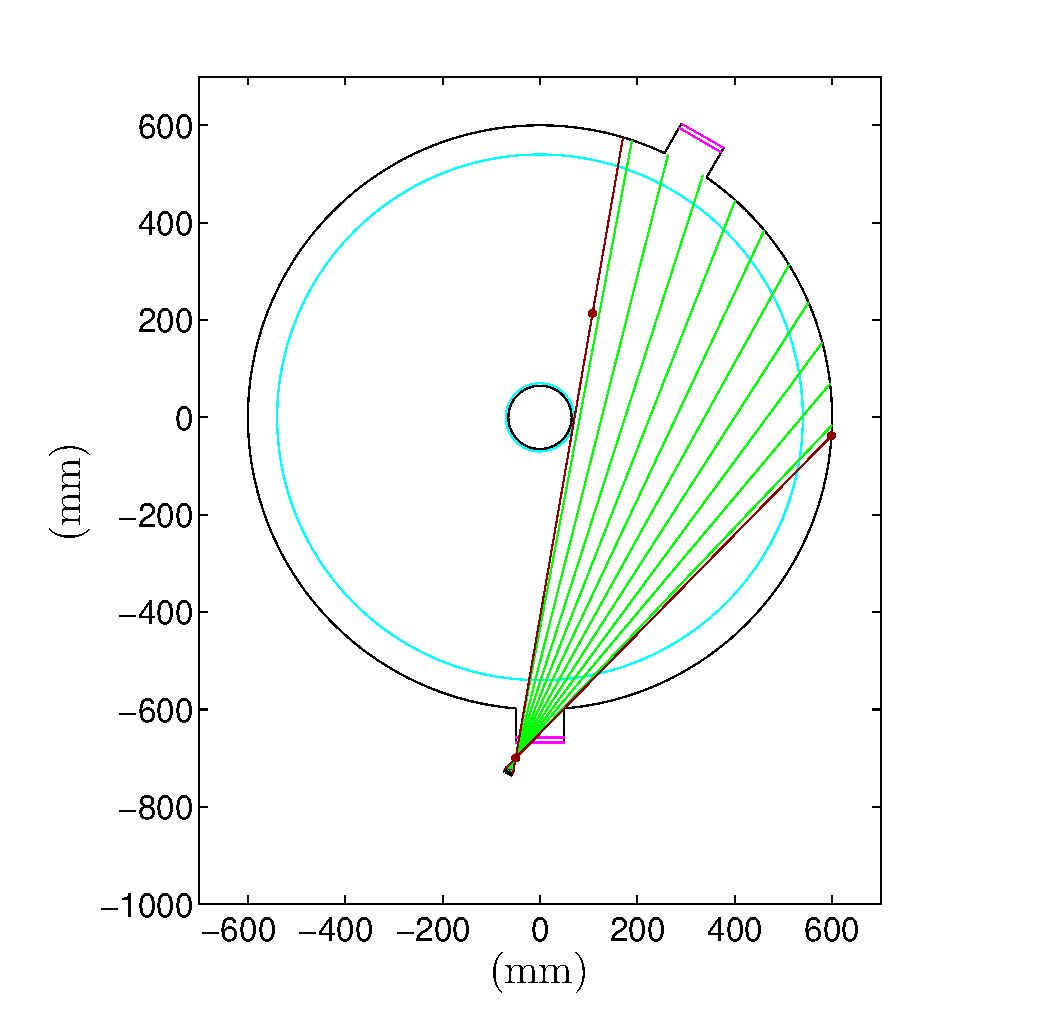
\includegraphics[width=\textwidth]{chords_conf.pdf}
    \caption{赤道面 10 通道测量路径优化}
    \label{fig:chap05:chords-conf}
  \end{subfigure}
  \\[1em] %\hspace{0.03\textwidth}
  \begin{subfigure}{0.6\textwidth}
    \setcaptionwidth{\textwidthswap}
    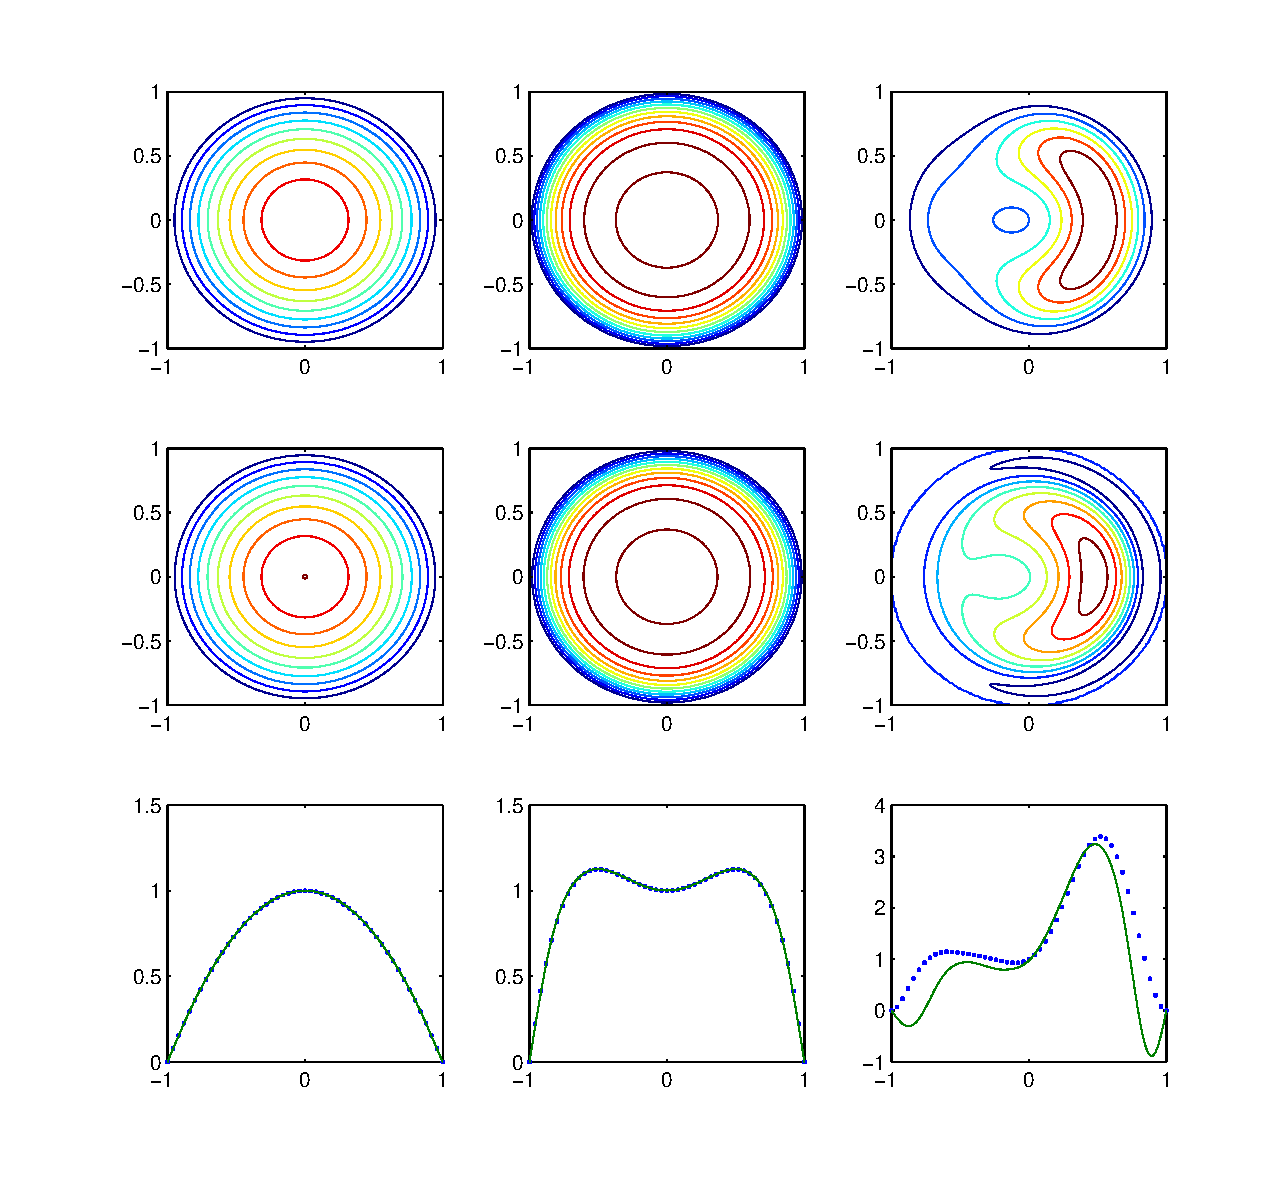
\includegraphics[width=\textwidth]{testplot.pdf}
    \caption{空间反演重建预研结果。第一列为对称分布;第二列为中空对称分布;第三列为非对称分布。第一行为假设分布参数等高线图;第二行为重建结果;第三行为水平中心线的假设分布与重建结果的对比,点为假设的分布,线为重建结果。}
    \label{fig:chap05:test-plot}
  \end{subfigure}
\end{center}
  \caption{SUNIST 中多通道光谱诊断测量预研}
  \label{fig:chap05:pda-measuring}
\end{figure}


3)无空间分辨诊断能力

本课题开展的光谱实验为赤道面上的单通道测量,不具备空间分辩诊断能力。在将来的工作中,可以在赤道面内安装具有多道测量能力的光电二极管阵列,并通过计算机断层重建技术实现赤道面内等离子体的光谱辐射率的空间分布测量,进而使用本文建立的谱线比法获得等离子体参数的空间分布诊断测量。我们对这种测量技术进行了预研,如图 \ref{fig:chap05:chords-conf} 所示为经优化后,在赤道面采用 10 通道光电二极管阵列测量时的最佳测量路径设计图。图 \ref{fig:chap05:test-plot} 所示为在不同的等离子体参数分布假设下,
使用基于空间傅立叶 -- 贝塞尔展开(Fourier–Bessel Basis Expansions)技术
\cite{Cormack1963:1,Cormack1964:2,WangLing1991:RadonTransform,RuanHuailin:Tomography}对三种不同等离子体参数假设分布情况的重建结果。


4)光谱诊断工作的丰富和深入

由图 \ref{fig:chap04:spectromgram-light-dbp10} 可见,原子谱线信号与等离子体磁信号具有一致的涨落行为,这说明对原子谱线辐射的分析可能会成为诊断等离子体磁流体力学行为的手段。在未来的研究中可以尝试在不同的位置同时测量等离子体的谱线辐射,尝试使用与磁探针信号相同的方法\cite{ZengLong2010:Thesis}分析其信号,这将会成为未来丰富和深入光谱诊断工作的突破口。

%SUNIST 实验基础方面
%
%? 不足:基于炮与炮之间重复放电测量,无法完全保证条件相同
%
%? 后续工作:建立新的实验设备,实现放电时谱线比的同时测量
